\section{Overview}

An automated regression test suite for any \boxlib\ code
exists in {\tt BoxLib/Tools/RegressionTesting/} as {\tt regtest.py}.
The test suite consists of a set of problem definitions (e.g., the
build directory, inputs files, etc.) and source locations for the
building blocks of the application.

When the suite is run the first time, the plotfiles created at the end
of each problem's execution are stored as a benchmark.  After this
initialization, each subsequent run of the test suite compares the
current output of the code, level-by-level and zone-by-zone to the
stored benchmarks (using the {\tt fcompare.f90} routine in {\tt
  BoxLib/Tools/Postprocessing/F\_Src/}).  Any differences are flagged as errors.
A web page report is generated by the test suite and provides a
history of the regression testing.  Many different types of tests
are supported, including:
\begin{itemize}
\item Single-processor and parallel tests (MPI and/or OpenMP)
\item compilation-only tests
\item self-tests (problems that determine by themselves whether they were successfully)
\item testing the checkpoint / restart capability
\item debug-mode tests
\end{itemize}

\begin{figure}[t]
\centering
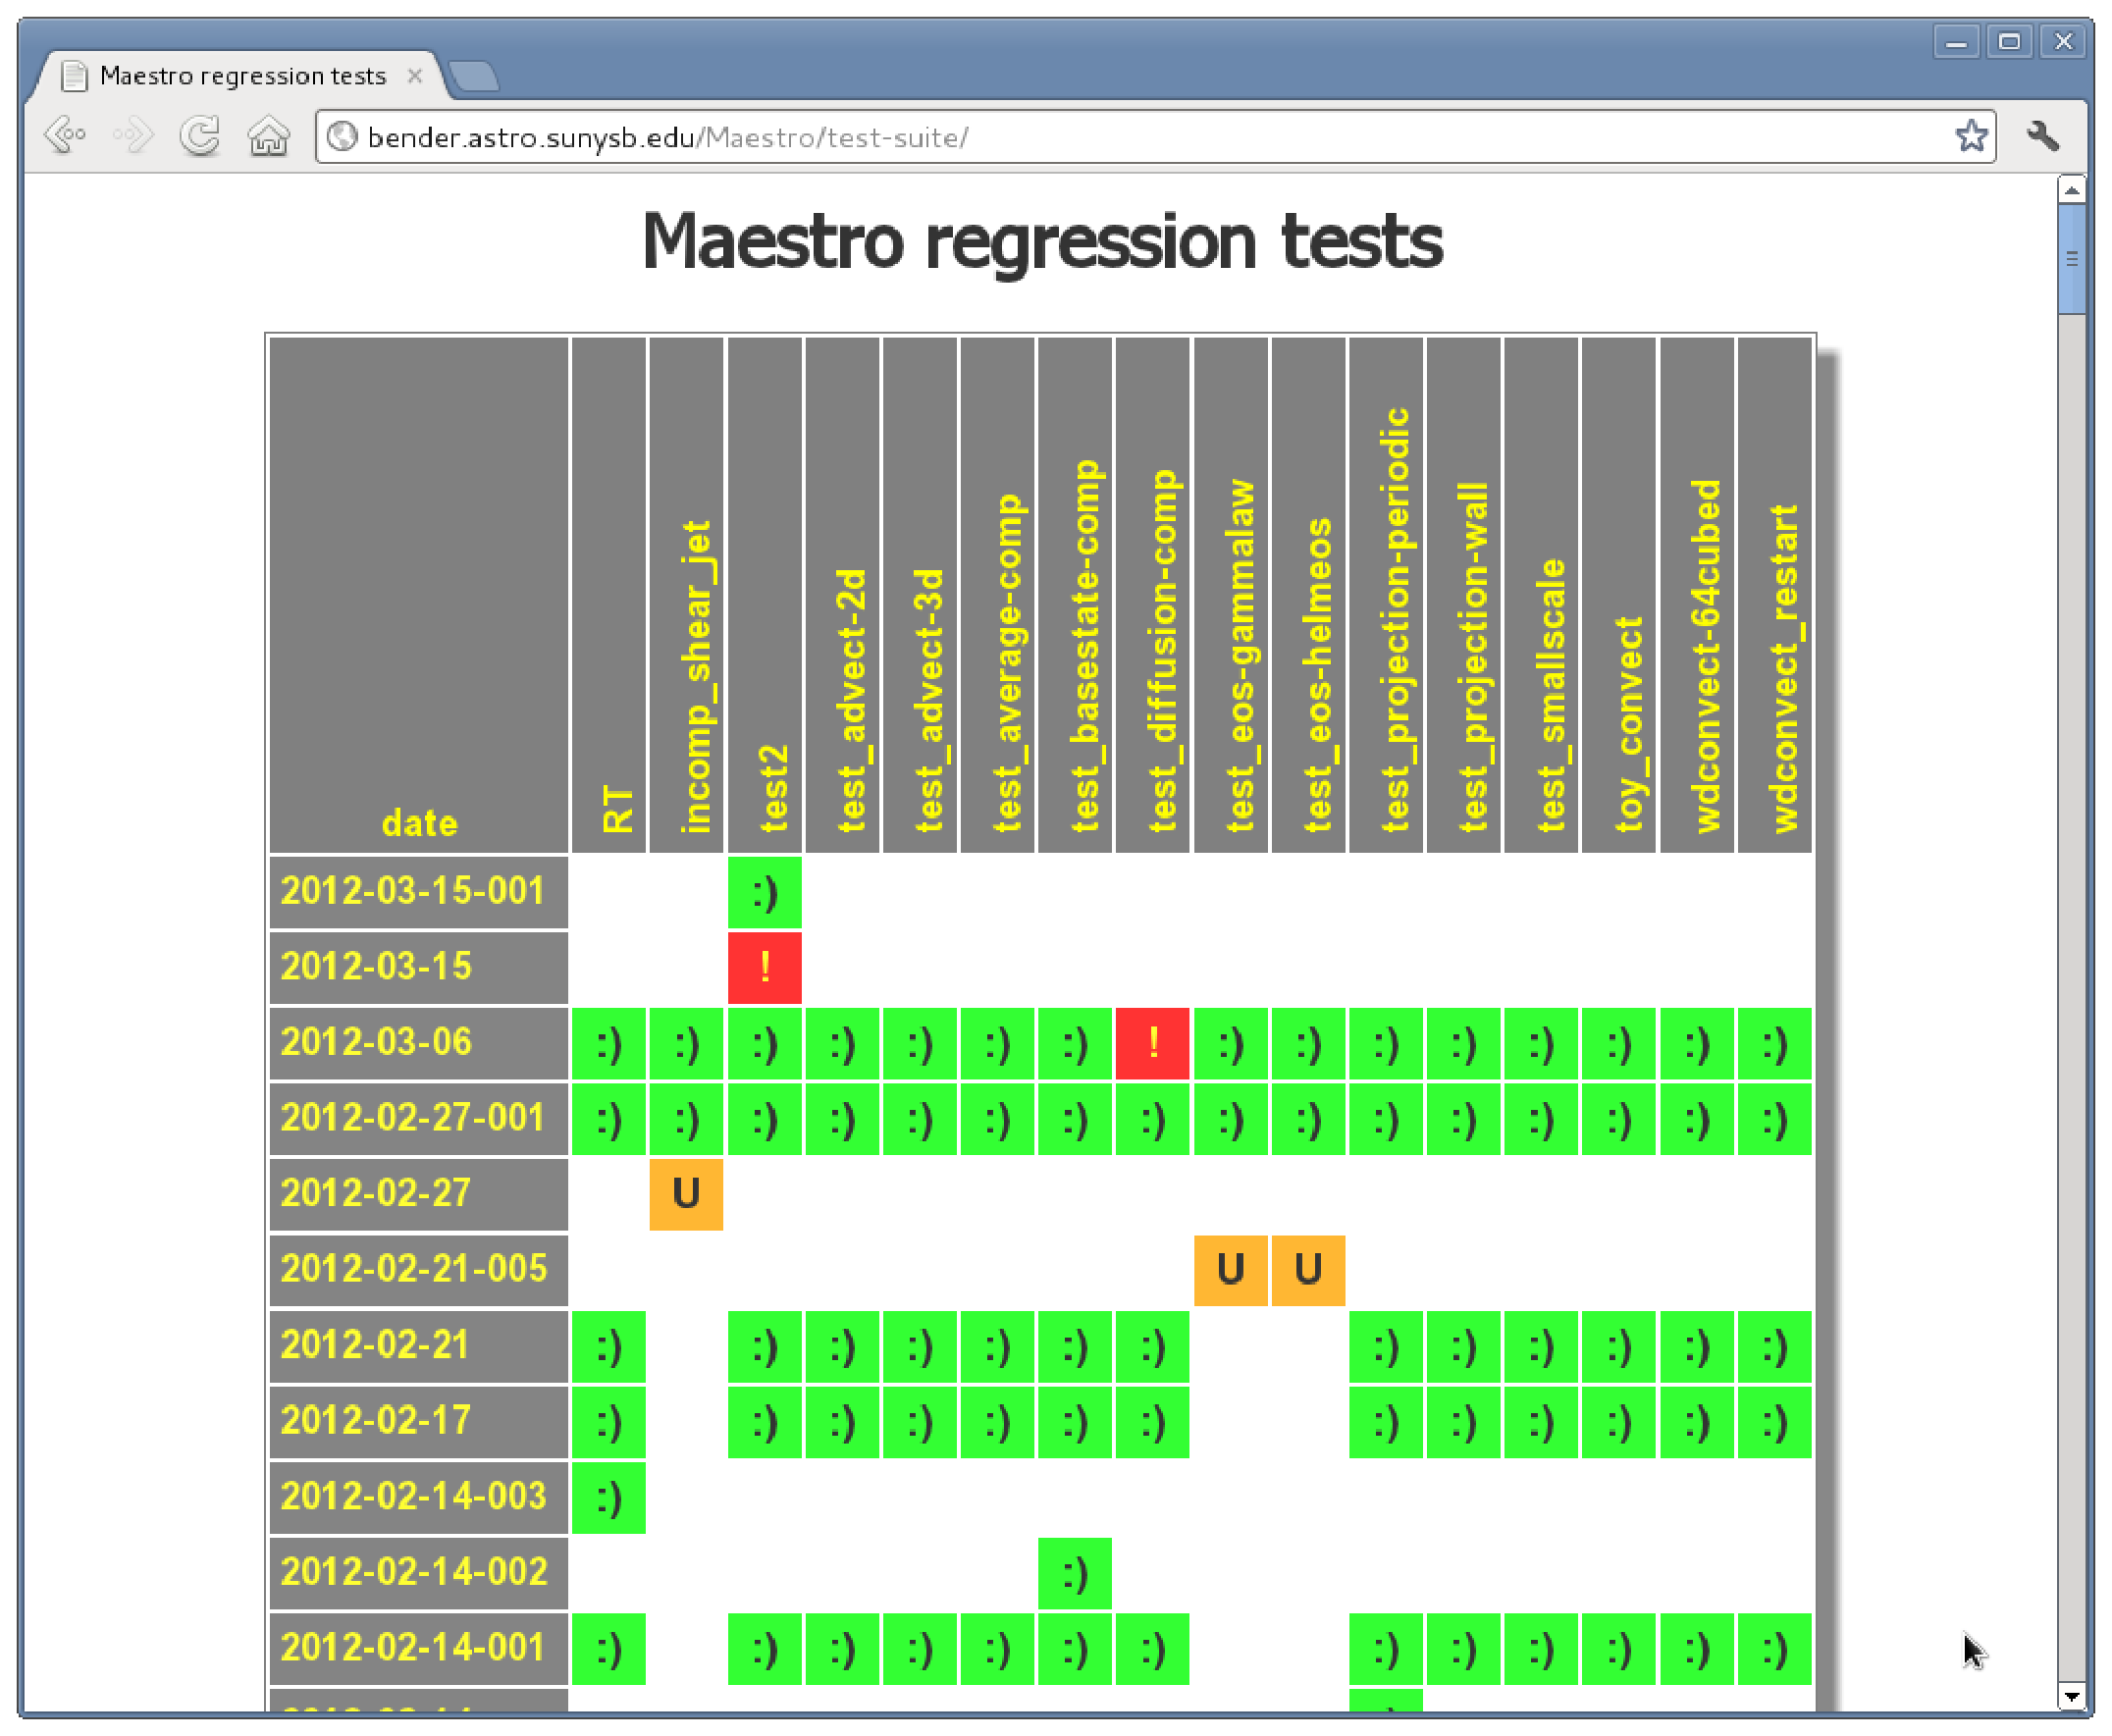
\includegraphics[width=5.0in]{testsuite}
\caption{\label{fig:test_suite_main} Main test suite results page.  Each
row indicates a single test suite run, arranged by date, and each column
indicates a different test problem. }
\end{figure}

\section{Test Suite Inputs File}

The inputs file for the test suite separates the problems into
sections (blocks).  There are several required sections: {\tt main},
{\tt BoxLib}, and {\tt source}, along with at least one problem
definition.  Some applications use source from multiple repositories,
so extra source repos are named {\tt extra-}{\ttfamily {\em sourcename}}.

Each of these section names appears in a heading delineated with {\tt [ ]}.
Beneath the heading a number of options that apply to that section.

\subsection{Suite-wide options}

An example of the {\tt [main]} block from {\tt Maestro-tests.ini} is:
\begin{lstlisting}
[main]
testTopDir     = /home/zingale/gfortran-testing/
webTopDir      = /home/www/Maestro/test-suite/gfortran-suite/

sourceTree = F_Src

suiteName = Maestro

reportActiveTestsOnly = 1

FCOMP = gfortran
add_to_f_make_command = TEST=t FSANITIZER=t

numMakeJobs = 4

purge_output = 1

summary_job_info_field1 = Network
summary_job_info_field2 = EOS

MPIcommand = mpiexec -n @nprocs@ @command@

globalAddToExecString = --single_prec_plotfiles F
\end{lstlisting}

The first group of options define the directories that the test suite
uses:
\begin{itemize}
\item {\tt testTopDir}: the directory that the suite should use as its
  root directory for running the tests
\item {\tt webTopDir}: the directory in which to place the web output.
\end{itemize}

For output, some descriptive options come next:
\begin{itemize}
\item {\tt suiteName}: the prefix to use on output directories---it
  does not need to match the program name
\item {\tt reportActiveTestsOnly}: whether to show all the tests on
  the web output known  to the suite throughout its history, or
  only the ones that are currently defined in the input file.
\end{itemize}

The source tree for \boxlib\ (Fortran or C++) and compilers to use are set
as:
\begin{itemize}
\item {\tt sourceTree}: set to {\tt F\_Src} for the Fortran
  \boxlib\ framework (appropriate for the \maestro\ example here). For
  a C++ \boxlib\ code, we'd set it to {\tt C\_Src}.
\item {\tt FCOMP}: sets the Fortran compiler to use---this will
  override what is listed in any {\tt GNUmakefile} to ensure that the
  compiler stays consistent in the tests.
\item {\tt COMP}: sets the C++ compiler to use---only needed for C++
  \boxlib\ codes
\item {\tt add\_to\_f\_make\_command}: this is an options to the make
  command we wanted added for every test.  Here we turn on the
  \boxlib\ {\tt TEST} features.
\item {\tt numMakeJobs}: tells the suite how many parallel build
  jobs to do at once (through the {\tt make -j N} command)
\end{itemize}

Finally, there are several parameters that describe how to run the code
\begin{itemize}
\item {\tt MPIcommand}: specify the generic manner in which to run an
  MPI program on the target system.  If present, the string {\tt
    @host@} in the {\tt MPIcommand} will be substituted by the {\tt
    MPIhost} string by the test suite.  Similarly the {\tt @nprocs@}
  string will be substituted by the number of processors, which is set
  on a problem-by-problem basis.  Finally, the {\tt MPIcommand} should
  include the string {\tt @command@}, which is where the
  \maestro\ executable and inputs file will be substituted.  For
  single processor runs, these options are ignored.
\item {\tt globalAddtoExecString}: an option to append to the
  executable string after the exectuable name and inputs file.  For
  example, here we override the parameter {\tt single\_prec\_plotfiles}
  which may be set in the problem's input file to ensure double
  precision output
\end{itemize}

There are a few additionally options, including those for sending
e-mail upon test completion or posting to a slack channel---see the full {\tt Maestro-tests.ini} for these.

\subsection{Sources}

The test suite expects that all the source code is in a git repo (or
repos).  The most important section is {\tt [BoxLib]}:
\begin{lstlisting}
[BoxLib]
dir = /home/zingale/gfortran-testing/BoxLib/
branch = development
\end{lstlisting}
This simply sets what directory to use for BoxLib and what git branch.
For applications, we will also have a main source---this will be the
default location that the suite looks to for building tests:
\begin{lstlisting}
[source]
dir = /home/zingale/gfortran-testing/MAESTRO/
branch = development
\end{lstlisting}
Any additional git repos that are needed can also be specified, e.g.,
{\sf Maestro} needs an additional repository called {\tt
  Microphysics}:
\begin{lstlisting}
[extra-Microphysics]
dir = /home/zingale/gfortran-testing/Microphysics/
branch = "development"
comp_string = MICROPHYSICS_HOME=@self@
\end{lstlisting}
Here we see an additional option: {\tt comp\_string} will always be
added to the make line, and in this case will set the variable {\tt
  MICROPHYSICS\_HOME} to the {\tt dir} listed in this section.

If an extra directory should also be used as a place to build tests,
then you need to supply the option {\tt build=1} in the section.

When the test suite is run, it will do a pull in each of the git repos
defined in the source sections and then checkout the requested branch.
It will also compare the branch name against a default branch (which
defaults to {\tt "development"}, and if any branch is not the default,
the master test webpage will put an asterisk next to the date to
indicate that it used an alternate branch.

\subsection{Problem-specific options}

Each problem to be run by the test suite gets its own block.  For
example, a test listing for the {\tt test2} problem might look like:

\begin{lstlisting}
[test2]
buildDir = TEST_PROBLEMS/test2/
inputFile = inputs_2d
aux1File = model.hse.cool.coulomb
link1File = helm_table.dat
dim = 2
doVis = 1
visVar = "tfromp"
compileTest = 0
restartTest = 0
useMPI = 1
numprocs = 4
\end{lstlisting}

Here {\tt test2} contained inside the {\tt []} is the name of the
problem, as the test suite will refer to it.  The options
for this test are then:
\begin{itemize}
\item {\tt buildDir}: th path beneath {\tt sourceDir} where the {\tt
  make} command should be executed.

  If instead we are building in the {\tt extraBuildDir}, then we would
  set {\tt useExtraBuildDir = 1}, and {\tt buildDir} will be relative
  to the extra build source directory.

\item {\tt inputFile}: the inputs file to use with the exectuable

\item {\tt aux1File}, {\tt aux2File}, {\tt aux3File}: any necessary
  auxillary files that need to be in the run directory (e.g., for C++
  \boxlib, the {\tt probin} file).

  Note that {\tt inputFile} and {\tt aux?File} are specified relative
  to the {\tt buildDir}.

\item {\tt dim}: the problem's dimensionality.

\item {\tt link1File}, {\tt link2File}, {\tt link3File}: these work
  like the {\tt aux?File}s, but instead of copying the specified file
  into the run directory, a symbolic link is made.

\item {\tt useMPI}: set to {\tt 1} if we are running parallel with
  MPI.  In this case, we also need to set {\tt numprocs} to the number
  of processors.

\item {\tt useOMP}: set to {\tt 1} if we are running parallel with
  OpenMP.  In this case, we also need to set {\tt numthreads} to the
  number of OpenMP threads
\end{itemize}

Less commonly used options include:
\begin{itemize}
\item {\tt compileTest}: set to {\tt 1} if we only want to test compiling
  the code, not running it.

\item {\tt restartTest}: set to {\tt 1} if we wish to test the
  checkpoint/restart capability.  In this case, we also set {\tt
    restartFileNum} to the number of the checkpoint file to restart
  from.  The suite will run the problem as usual and then restart from
  the specified checkpoint and run to completion again.  The output
  from the initial run will then be compared to the output from the
  restart.  In a restart test, there is no stored benchmark.

\item {\tt selfTest}: Some problems don't output plotfiles, but
  instead check internally whether they are successful.  For these,
  set {\tt selfTest} to {\tt 1}, and set {\tt stSuccessString} to the
  string output to look for at the end of the test to determine if it
  was successful.

\item {\tt doVis}: set to {\tt 1}, this enables simple visualization
  to the test suite webpage.  You need to set {\tt visVar} to the name
  of the plotfile variable to visualize.  An image of that field from
  the last plotfile will be appended to the problem's test webpage.

\item {\tt compareFile}: Ordinarily, the test suite uses the last
  plotfile output to compare to.  To force the comparison to a
  specific file, set {\tt compareFile} to the name of the file to
  compare to.

\item {\tt addToCompileString}: provides a means to override some of
  the options in the problem's {\tt GNUmakefile} (e.g.\ use a
  different reaction network).  Set {\tt addToCompileString} to the
  string to add to the {\tt make} line that compiles the problem.
\end{itemize}

If the test requires the source to be build in a directory other 
than that referred to by the {\tt [source]} section, then you
need to add the option
\begin{lstlisting}
extra_build_dir = name
\end{lstlisting}
where {\tt name} is the part of the section {\tt [extra-name]} 
that defines the repo.

\section{Initializing the Test Suite}

The first time you run the test suite there are no benchmark files to
compare to.  Once you generate an inputs file, as described above, you
would simply run the suite as:
\begin{verbatim}
 ./regtest.py  --make_benchmarks "initial run" ./Maestro_tests.ini
\end{verbatim}
The string following {\tt --make\_benchmarks} is simply a comment that
will be added to the web report.  This command creates three output
directories, using the {\tt suiteName} as the prefix.
\begin{itemize}
\item {\tt suiteName-tests/} is where the tests are run.  Each time the
  test suite is run, a subdirectory, based on the date, is created,
  with a subdirectory for each test.  All the files necessary to run
  the test are copied into the test subdirectory.

\item {\tt suiteName-web/} is where the web-based reports for the test
  are generated.  The master webpage is {\tt
    suiteName-web/index.html}.

  Note: if {\tt webTopDir} is set in the {\tt [main]} option block, we
  use that instead

\item {\tt suiteName-benchmarks} is where the test benchmark files are
  stored.  This are used for comparison to the current output.
\end{itemize}



\section{Regular Use}

Once the initial benchmarks are created, you can compare the current
version of the code to the stored results by simply doing:
\begin{verbatim}
./regtest.py ./Maestro_tests.ini
\end{verbatim}
This will do a git update in all the source repos (including \boxlib),
generate {\tt ChangeLog} files listing all of the git comments for the
code, build the test comparison tools, and then loop over each test,
building and running the executable and comparing the output to the
benchmarks as required.

Upon completion of all the runs, a web page for this invocation of the
test suite will be generated as well as pages showing the details for
each of the problems run.  Test failures indicate that the current
output does not match the stored benchmarks.

There are additional runtime options to run only tests of a certain
dimensionality, those that previously failed, etc.  Typing {\tt
  ./regtest.py} with no options will give a description of these
options.


\section{Updating Benchmarks}

A test failure means that the current version of the code gives a
different answer than the stored benchmark.  A test can fail either
because a bug was introduced into the code or a bug was fixed or new
feature introduced.

If a bug was introduced into the code recently, then by examining the
test history you can determine the time period in which the bug was
introduced.  The {\tt ChangeLog}s linked to on each test date's webpage
will list all the changes committed to git up to that point, which is
useful for tracking down the bug.  Once the bug is fixed, rerunning
the suite should generate a `pass'.

If a bug was fixed or a new feature was introduced, and you are
confident that the latest output is correct, then you can tell the
test suite to update the benchmarks.  If you want to do this for all
the test problems, you would do:
\begin{verbatim}
./regtest.py --make_benchmarks "X bug fixed" ./Maestro_tests.ini
\end{verbatim}
where the string after ``{\tt --make\_benchmarks}'' is a note that is listed
on the regression suite web page describing the reason for the benchmark
update.  Subsequent runs of the test suite will use the new benchmarks.
If you only want to update the benchmarks of a single test, then you
can use the ``{\tt --single\_test test}'' flag on the commandline, where
{\tt test} is the name of the test to update.

Finally, if you just want to rerun the tests the previously failed,
you can use the {\tt --redo\_failed} option.
